\documentclass{article}

\usepackage{tabularx}

\usepackage{graphicx}
\graphicspath{ {img/} }


\title{RAID Configuration: Pragmatic Selection Strategies}
\author{Marcel Schubert}
\date{30.03.2024}

\begin{document}
\maketitle

\section*{Introduction}
Choosing the right configuration for the logical disks
of your systems is no trivial task. But it is still one, many technicians are faced with. 
\\ \\
The aim of this report is to offer practical approaches for selecting the appropriate configuration for a specific task, without delving into the underlying technical intricacies. It adopts a narrow perspective, focusing solely on factors such as reliability, capacity, cost, and performance, while disregarding considerations like access protocols or optimized implementations. Nevertheless, the provided information can serve as a foundation for calculating and comparing theoretical values, empowering readers to make more informed decisions or conduct additional research.
\\ \\
The methodology employed in this report is primarily based on the analysis of readily available information online. Due to the non-scientific nature of this approach, most of the information was not verified beyond basic plausibility checks. It's important to note that no quantifiable empirical measurements were conducted as part of this study.
\\ \\
The report is structured into five main parts. The first four sections provide essential information on comparing reliability, capacity, cost, and performance. In the final section guide, a straightforward overarching method is presented, along with additional vendor-specific information contained within this chapter.
\pagebreak
\tableofcontents
\pagebreak
\section{Reliability}
Due to the complexity of real-life situations, simple numeric methods may not provide conclusive results. For instance, when considering the average failure time of a single drive and then extrapolating it across a storage group, the probability of a drive failing will evidently increase significantly with a higher number of drives. Analytically defining this change is challenging due to its dependency on various factors. For example, it's frequently observed that drives from the same production batch may fail together in short succession, making it difficult to determine such factors definitively. \cite{cmu:raidhighperf}
\\ \\
Still, if one wants to get a simple overview, formulas are included for the failure calculation for RAID-5
and RAID-6.
\begin{equation}
    \label{eq:r5-mttf}
    \frac{MTTF^2(disk)}{N*(G-1)*MTTR(disk)}
\end{equation}
Equation \ref{eq:r5-mttf} gives a way to calculate the mean time to failure
of RAID-5 arrays.
Where \(MTTF(disk)\) is the mean time of failure of a single disk
\(N\) is the number of disks and \(G\) is the size of the arrays.
The equation assumes no correlated failures, that means that
this simple model assume all disks are independent.
The same calculation looks slightly different for RAID-6 as seen
in eqation \ref{eq:r6-mttf}. \cite{cmu:raidhighperf}
\begin{equation}
    \label{eq:r6-mttf}
    \frac
    {MTTF^3(disk)}
    {N*(G-1)*(G-2)*MTTR^2(disk)}
\end{equation}
An overview of the hardware failures that can occur without disrupting service 
is presented in Table \ref{tab:reliability}.
It's worth noting that in RAID-1, the impact of a failure largely
depends on luck regarding the location of the failure.
If the stripes are favorably replicated, multiple drives
may be able to fail without service disruption. \cite{uw:raid} 
\begin{table}[h]
    \begin{tabularx}{\textwidth}{l|X|X|X|X|X|X}
        \textbf{Level} &
        Failures \\
        \hline
        0 & 0 \\
        1 & 1 or \( \frac{n}{2} \) \\
        2 & 1 \\
        3 & 1 \\
        4 & 1 \\
        5 & 1 \\
        6 & 2 \\
       \end{tabularx}
    \caption{Amount of drives able to fail without array service degradation \cite{uw:raid}}
    \label{tab:reliability}
\end{table}
\pagebreak
\section{Capacity}
A comparative capacity calculation can relatively easily be done using table \ref{tab:capacity}.
\begin{table}[h]
    \begin{tabularx}{\textwidth}{l|X|X|X|X|X|X}
        \textbf{Level} &
        Space Efficiency \\
        \hline
        0 & n \\
        1 & \( \frac{n}{2}\)\\
        2 & \( (1-\frac{1}{n}*log_2(n+1))*full_caption \) \\
        3 & n-1 \\
        4 & n-1 \\
        5 & n-1 \\
        6 & n-2 \\
       \end{tabularx}
    \caption{Coefficient of the space multiplication (smallest disk). \cite{uw:raid} The calculation of RAID-2 was
    derived from Chen et al., Alagappan and wikipedia. \cite{cmu:raidhighperf}\cite{uw:raid}}
    \label{tab:capacity}
\end{table}
\pagebreak

\section{Cost}
An economic comparison can be facilitated using the matrix illustrated in Table \ref{tab:economics}.
It's practical to assess the cost relative to RAID level-0, as it represents the configuration with the 
lowest cost/efficiency rating. To compare the various options, utilize \( N = \textnormal{ Number of disks}\)
and \(\max\left(x,y\right)\) as the known max function with \( x, y \in R \).
In this calculation, "small" denotes I/O requests of one striping unit, while "large" 
denotes I/O requests of one full stripe (one stripe unit from each disk in an error-correction group). 
The overview can be seen in figure \ref{fig:costthroughput} which 
plots this against arrays of different sizes. \cite{cmu:raidhighperf}
\begin{table}[h]
    \begin{tabularx}{\textwidth}{l|X|X|X|X|X}
        \textbf{Level} &
        Small Read &
        Small Write &
        Large Read &
        Large Write &
        Storage Efficiency \\
        \hline
        0 & 1 & 1 & 1 & 1 & 1 \\
        1 & 1 & \( \frac{1}{2} \) & 1 & \( \frac{1}{2} \) & \( \frac{1}{2} \) \\
        3 & \( \frac{1}{N} \) & \( \frac{1}{N} \) & \( \frac{N-1}{N} \) & \( \frac{N-1}{N} \) & \( \frac{N-1}{N} \) \\
        5 & 1 & \( \max\left(\frac{1}{N},\frac{1}{4}\right) \) & 1 & \( \frac{N-1}{N} \) & \( \frac{N-1}{N} \) \\
        6 & 1 & \( \max\left(\frac{1}{N},\frac{1}{6}\right) \) & 1 & \( \frac{N-2}{N} \) & \( \frac{N-2}{N} \) \\
    \end{tabularx}
    \caption{Cost Throughput Comparison relative to RAID-0 \cite{cmu:raidhighperf}}
    \label{tab:economics}
\end{table}
\pagebreak
\begin{figure}[h]
    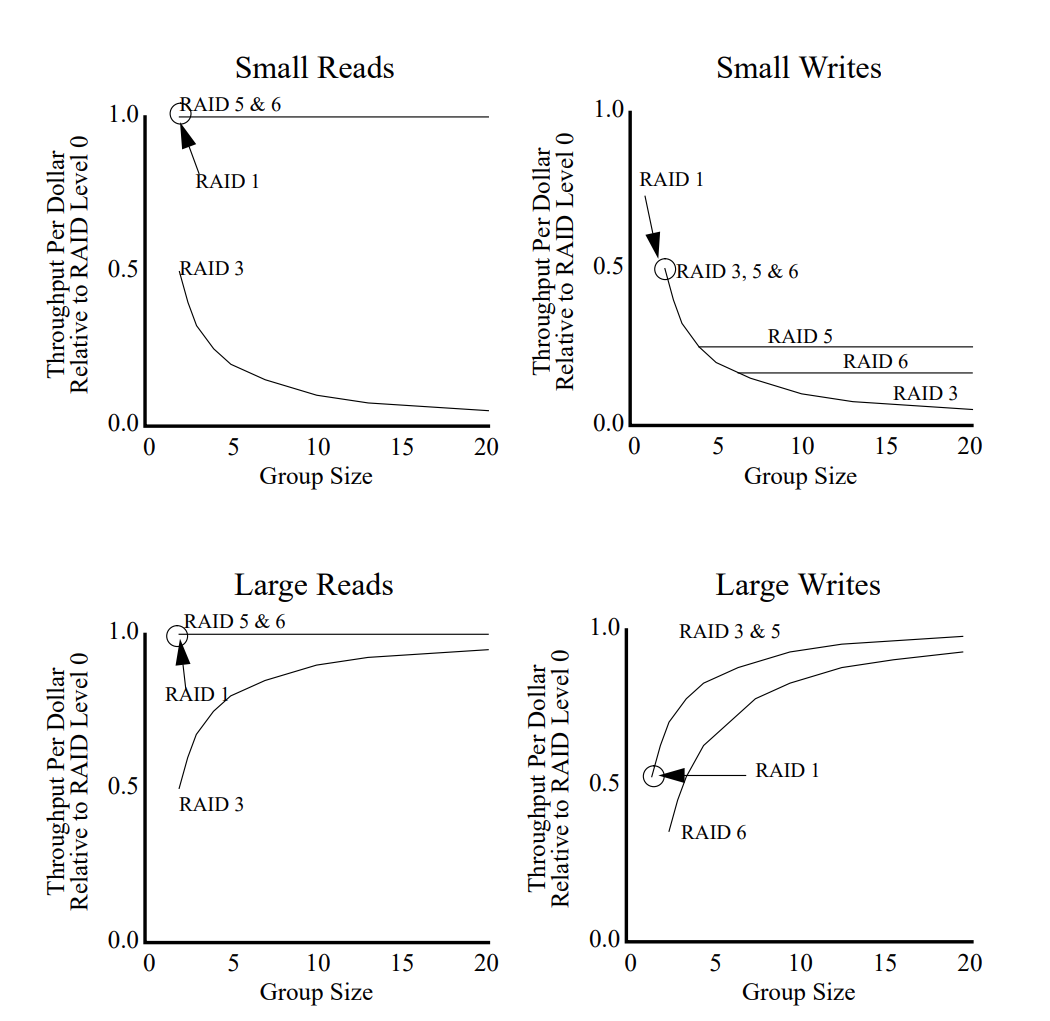
\includegraphics[width=\textwidth]{cost-troughput-comparison}
    \caption{Cost Throughput Comparison}
    \label{fig:costthroughput}
\end{figure}
\pagebreak
\section{Performance}
You can approximate the theoretical upper bound of performance using Table \ref{tab:perf}. 
The calculation considers only conceptual first-order factors. Despite this limitation, 
comparing these fundamental boundaries can still be beneficial for outlining performance expectations. 
The table provides coefficients that can be multiplied by the given drive metrics 
(random read, random write, sequential read, sequential write). 
It's important to note that this approach does not specify block sizes and
can be applied to average or median values. \cite{uw:raid}
\subsection{Nested RAID Configuraitions}
For nested RAID configurations, begin by calculating the values for a single group, and then iterate the calculation. Distribute the group size evenly across the total number of disks.

For instance, calculate the table for a single RAID-5 group first,
and then take those values and plug them back into the table again.
It's important to note that this approach does not include many optimizations typically implemented on platforms.
Again keep in mind, that this is only an approximation.
\begin{table}[h]
    \begin{tabularx}{\textwidth}{l|X|X|X|X|X|X}
        \textbf{Level} &
        sread &
        swrite &
        rread &
        rwrite &
        rlatency &
        wlatency \\
        \hline
        0 & n & n & n & n & 1 & 1\\
        1 & \( \frac{n}{2}\) & \( \frac{n}{2}\) & n & \( \frac{n}{2}\) & 1 & 1\\ 
        4 & n-1 & n-1 & n-1 & \( \frac{1}{2}\) & 1 & 2 \\ 
        5 & n-1 & n-1 & n & \( \frac{n}{4}\) & 1 & 2 \\
        6 & n-2 \cite{cmu:raidhighperf}& n-2 \cite{cmu:raidhighperf}& n \cite{cmu:raidhighperf}& \( \frac{n}{6} \) \cite{cmu:raidhighperf}& 1 \cite{cmu:raidhighperf}& 2 \cite{cmu:raidhighperf}\\
       \end{tabularx}
    \caption{Performance Calculation \cite{uw:raid}, The original talbe does not include RAID-6 so it was derived from Chen et al \cite{cmu:raidhighperf}}
    \label{tab:perf}
\end{table}
Also notice, that with increasing number of disks
the upper bound of the throughput can be amplified,
but generaly latency is not improved.
\subsection{Other Factors}
It's crucial to always refer to specific hardware and software documentation,
as theoretical speeds heavily rely on particular implementations.
Factors such as controller features, choice of algorithms,
and caching mechanisms play an immense role in determining actual performance.
In the most general case, we assume that these factors scale with a constant value.

Additionally, it's important to consider other variables that can impact performance,
such as network latency, system workload, and environmental conditions.
By thoroughly understanding the specific characteristics of the hardware and software being used,
one can better optimize configurations and make more accurate performance assessments.
Furthermore, staying informed about updates and advancements in technology
can help ensure that systems are operating at their highest potential.
\pagebreak
\section{Guide}
For a quick comparison, utilize the Microsoft Excel 
workbook "raid-workbook.xlsx" provided with this report.
Input the dependent variables such as drive size and IO speeds, 
then delve deeper into analyzing the results. \cite{mas:workbook}
\subsection{HPE Smart Array}
HP provides various storage solutions, one of which includes the Smart Array Controllers,
offering distinct functionalities categorized into classes.
This section provides an overview and presents HP's insights on reliability, performance, and efficiency regarding these controllers.
\\ \\
The Smart Array Controllers are categorized into three main classes: S, E, and P.
S-Class serves as an entry-level product, offering a typical software RAID solution tailored for MS Windows environments.
E-Class controllers provide enterprise-level functionalities, although they may lack some high-performance optimizations like caching.
P-Class controllers are designed for performance optimization, 
offering typical performance-oriented functionalities along with optimizations such as caching and support for various interfaces.
For detailed information regarding the feature matrix, it's advisable to consult the documentation available online. \cite{hpe:sa-userguide}
\\ \\
In terms of performance, HP suggests considering that as fault tolerance improves, performance may decrease due to additional I/O overhead.
Additionally, HP notes that read performance is generally consistent across all RAID levels, except for smaller RAID 5 or 6 arrays. \cite{hpe:sa-userguide}
\\ \\
In their documentation, HP nearly presents identical theoretical numbers to facilitate a performance comparison.
They simplify their model based on the required number of write I/O operations.
\begin{itemize}
    \item RAID-0, 1x Steps IO 
    \item RAID-1/10, 2x Steps IO
    \item RAID-1/10 Triple, 3x Steps IO
    \item RAID-5, 4x Steps IO
    \item RAID-6, 6x Steps IO
\end{itemize}
This clearly demonstrates a significant similarity to the model utilized in the "Performance" chapter.
\\ \\
In terms of capacity considerations, HP advises taking into account that usable capacity diminishes
as fault tolerance improves, primarily due to the increase in parity data.
Moreover, they indicate that the usable capacity for RAID 10 and RAID 10 Triple remains consistent with larger arrays,
while for RAID 5, 50, 6, and 60, it tends to increase with larger arrays. \cite{hpe:sa-userguide}
\\ \\
\begin{figure}
    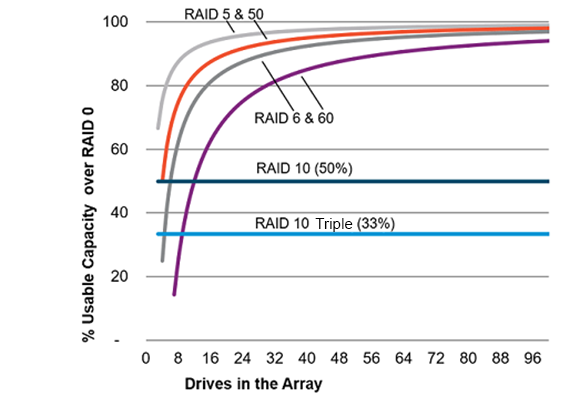
\includegraphics[width=\textwidth]{hp-storage-efficiency}
    \caption{HP Storage Efficiency \cite{hpe:sa-userguide}}
    \label{fig:hp-storage-efficiency}
\end{figure}
Figure \ref{fig:hp-storage-efficiency} shows a general plot of the storage efficiency development
over a increasing amount of disks. The plot assumes the group size 2 for RAID-50 and RAID-60. \cite{hpe:sa-userguide}
\\ \\
At last consider following suggestions by HP:
\begin{itemize}
    \item RAID 1/10 Triple: Optimize for fault tolerance and write performance.
    \item RAID 6/60: Optimize for fault tolerance and usable capacity.
    \item RAID 1/10: Optimize for write performance.
    \item RAID 5/50: Optimize for usable capacity.
\end{itemize}

\section*{Fun Facts}
It seems that RAID initially stood for "Redundant Array of Inexpensive Disks"
before evolving into the more widely recognized version, "Redundant Array of Independent Disks."
Source is: trust me brother; cannot be bothered to look it up.
\listoffigures
\listoftables
\bibliographystyle{ieeetr}
\bibliography{refs}
\begin{figure}[h]
    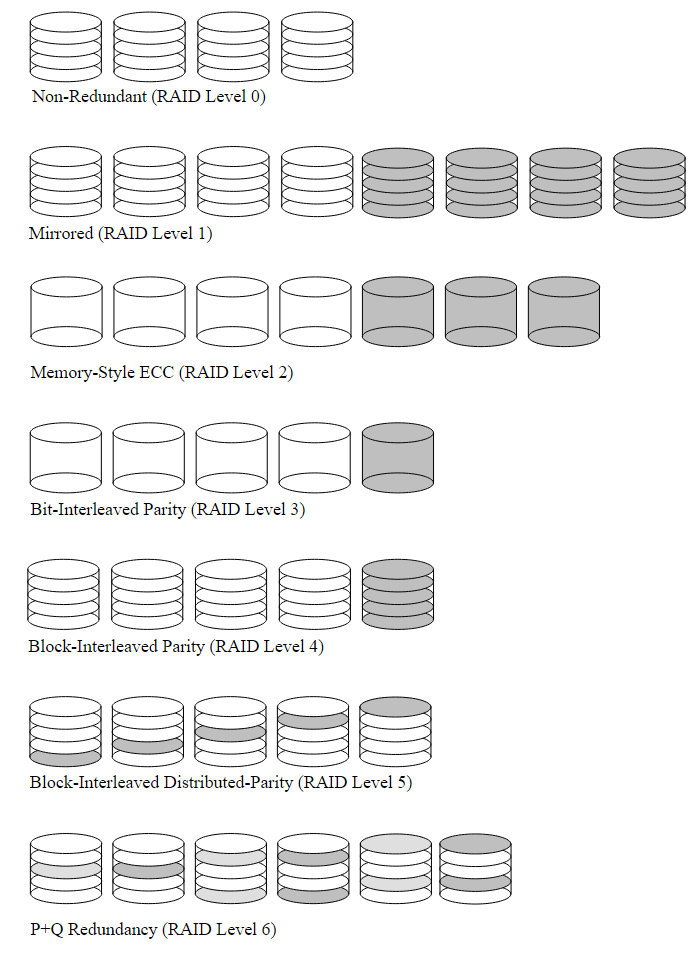
\includegraphics[width=\textwidth]{raid-overview}
    \caption{Raid Overview \cite{cmu:raidhighperf}}
    \label{fig:raid-overview}
\end{figure}
\end{document}